\section{Zadanie 5}
\subsection{Opis problemu}
Zadanie polegało na wygenerowaniu wykresów wielomianów interpolowanych z poniższych funkcji za pomocą wcześniej zaimplementowanych metod.
\begin{enumerate}
  \item $f(x) = |x|, [-1, 1], n = 5, 10, 15$
  \item $g(x) = \frac{1}{1 + x^2}, [-5, 5], n = 5, 10, 15$
\end{enumerate}
\subsection{Rozwiązanie}
Na poniższych rysunkach przedstawiłem wykresy dla funkcji $f(x)$ oraz $g(x)$ dla poszczególych $n = 5, 10, 15$ 
\begin{figure*}
  \begin{multicols}{2}
        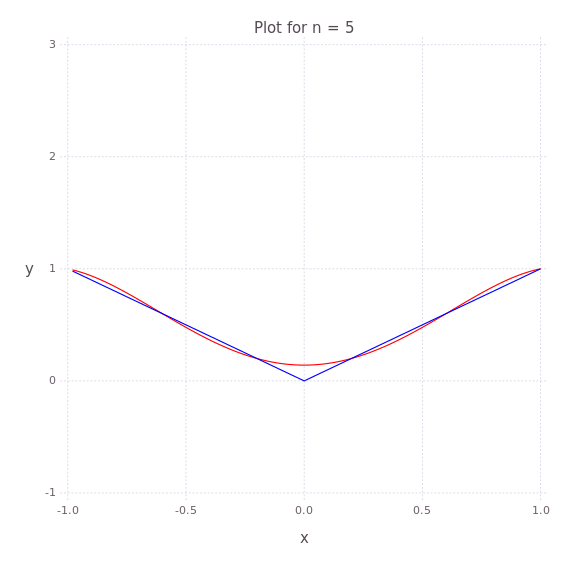
\includegraphics[width=\linewidth]{../task-6/plots/myplot-abs-5.png}\par 
        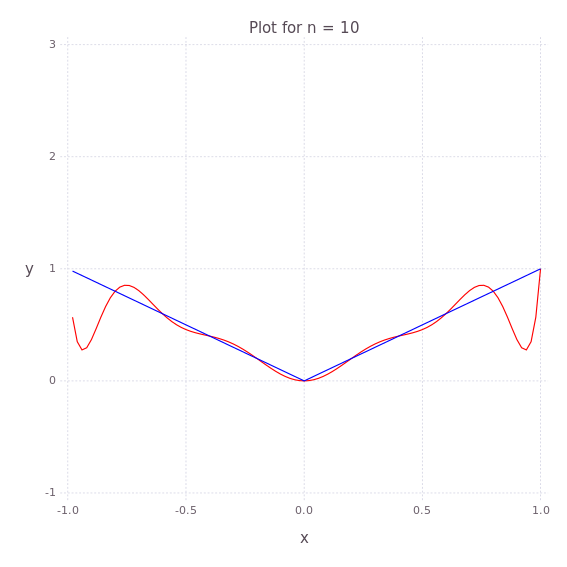
\includegraphics[width=\linewidth]{../task-6/plots/myplot-abs-10.png}\par 
    \end{multicols}
    \begin{multicols}{2}
        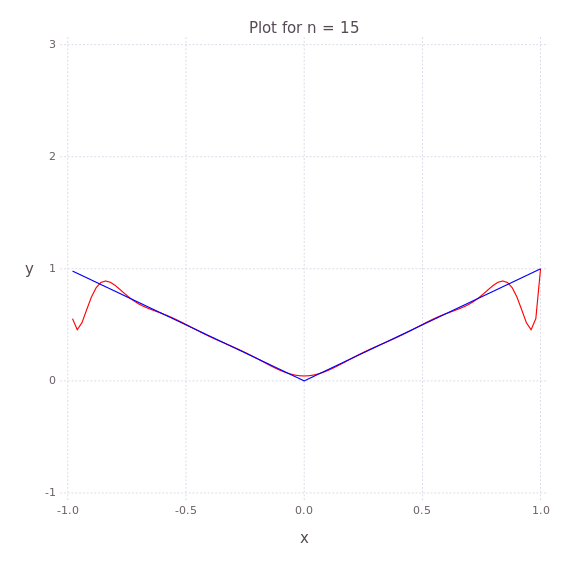
\includegraphics[width=\linewidth]{../task-6/plots/myplot-abs-15.png}\par 
    \end{multicols}
    \caption{Wykresy dla $f(x) = |x|$}    
\end{figure*}
\begin{figure*}
    \begin{multicols}{2}
        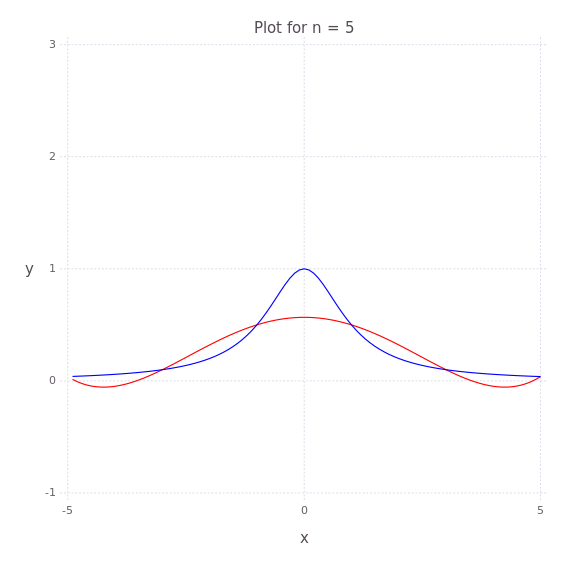
\includegraphics[width=\linewidth]{../task-6/plots/myplot-1x2-5.png}\par 
        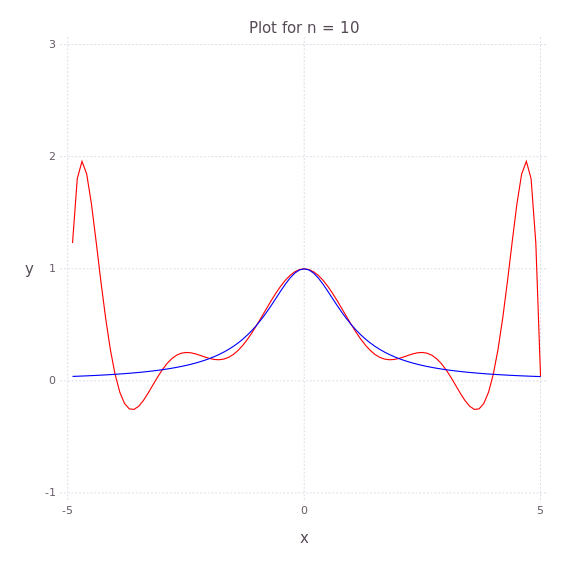
\includegraphics[width=\linewidth]{../task-6/plots/myplot-1x2-10.png}\par           
    \end{multicols}
    \begin{multicols}{2}
        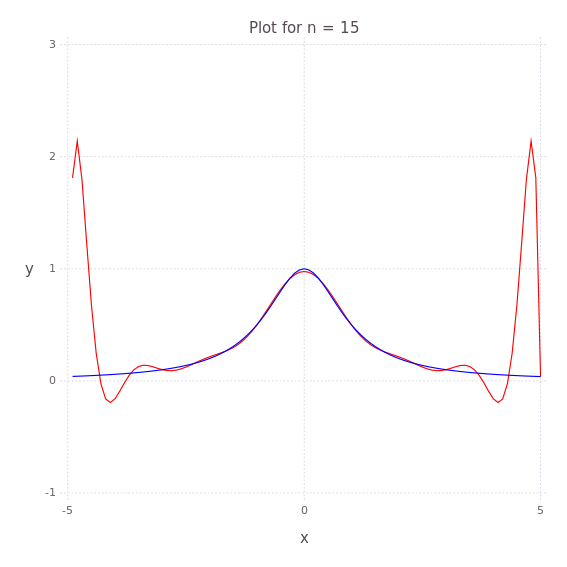
\includegraphics[width=\linewidth]{../task-6/plots/myplot-1x2-15.png}\par
    \end{multicols}
    \caption{Wykresy dla $g(x) = \frac{1}{1 + x^2}$}    
\end{figure*}
\subsection{Analiza wyników}
W przypadku tego zadania mieliśmy do czynienia z funkcjami, dla których wielomiany interpolacyjne są podatne na tzw. $\textsc{efekt Rungego}$. (pogorszenie jakości interpolacji mimo zwiększenia ilości węzłów) Efekt ten często występuje, gdy:
\begin{enumerate}
    \item interpolowana funkcja jest nieciągła
    \item funkcja odbiega znacząco od funkcji gładkiej\footnote{Funkcja gładka - funkcja ciągła i mająca pochodne wszystkich rzędów}
    \item wielomiany interpolujące mają wysokie stopnie, a odległość między więzłami jest stała
\end{enumerate}
W przypadku funkcji $f(x) = |x|$ dla $n = 5$ interpolacja nie była dokładna w okolicach $x = 0$, lecz bliska $f(x)$ na krańcach przedziału. Po zwiększeniu ilości węzłów do $n = 10$, wygenerowany wielomian był bardziej dokładny w centrum, lecz na krańcach pojawił się wyżej wspomniany efekt Rungego, który nie został zniwelowany dla $n = 15$. Powodem wystąpienia efektu był brak ciągłości funkcji oraz równe odstępy między poszczególnymi węzłami $x_i$. \\\\
Wielomian będący interpolacją $g(x) = \frac{1}{1 + x^2}$ dla $n = 5$ odbiega od rzeczywistego wykresu $g(x)$. Po zwiększeniu ilości węzłów do $n = 10$, interpolacja staje się bliższa wyjściowej funkcji w okolicach $x_i = 0$, lecz na krańcach przedziału pojawia się efekt Rungego. Zwiększając ilość węzłów do $n = 15$ efekt nie zniknął. Powodem wystąpienia efektu Rungego w tym wypadku była nieciągłość funkcji i jednakowa odległość między poszczególnymi węzłami 
\\\\
W celu zniwelowania błędów wynikających z efektu Rungego - dużych oscylacji wielomianu interpolacyjnego na krańcach przedziału - należy gęściej upakować węzły na tych krańcach przedziału interpolacji, np. wykorzystując $\textsc{wielomiany Czybyszewa}$, których miejsca zerowe zagęszczają się na krańcach.